\documentclass[12pt,letterpaper,oneside,reqno]{amsart}
\usepackage{amsfonts}
\usepackage{amsmath}
\usepackage{amssymb}
\usepackage{amsthm}
\usepackage{float}
\usepackage{mathrsfs}
\usepackage{colonequals}
\usepackage[font=small,labelfont=bf]{caption}
\usepackage[left=1in,right=1in,bottom=1in,top=1in]{geometry}
\usepackage[pdfpagelabels,hyperindex,colorlinks=true,linkcolor=blue,urlcolor=magenta,citecolor=green]{hyperref}
\usepackage{graphicx}
\linespread{1.7}
\emergencystretch=1em

\newtheorem{thm}{Theorem}[section]
\newtheorem{example}[thm]{Example}
\newtheorem{definition}[thm]{Definition}

% free foot note
\let\svthefootnote\thefootnote
\newcommand\freefootnote[1]{%
    \let\thefootnote\relax%
    \footnotetext{#1}%
    \let\thefootnote\svthefootnote%
}


\title[Software product Release flow: A proposal]
{Software product Release flow: A proposal}
\author[Petro Kolosov]{Petro Kolosov}
\address{Software Developer, DevOps Engineer}
\email{kolosovp94@gmail.com}
\urladdr{https://kolosovpetro.github.io}
\date{\today}
\keywords{
    Software engineering,
    DevOps,
    Software release,
    GitHub flow,
    GitLab flow,
    Azure DevOps,
    Azure pipelines,
    Semantic versioning,
    GitVersion,
    CI/CD
}
\hypersetup{
    pdftitle={Release Flow Proposal},
    pdfsubject={
        Software engineering,
        DevOps,
        Software release,
        GitHub flow,
        GitLab flow,
        Azure DevOps,
        Azure pipelines,
        Semantic versioning,
        GitVersion,
        CI/CD
    },
    pdfauthor={Petro Kolosov},
    pdfkeywords={
        Software engineering,
        DevOps,
        Software release,
        GitHub flow,
        GitLab flow,
        Azure DevOps,
        Azure pipelines,
        Semantic versioning,
        GitVersion,
        CI/CD
    }
}
\begin{document}
    \begin{abstract}
        Your abstract here.
    \end{abstract}

    \maketitle

    \tableofcontents
    \freefootnote{Sources: \url{https://github.com/kolosovpetro/ReleaseFlowProposal}}


    \section{Introduction} \label{sec:introduction}
    Release flow is a set of steps to perform to release upcoming version of software product.
Main aim of this document is to present simple and working model of software release
using semantic versioning~\cite{SemanticVersioning}, azure pipelines,
and mainline development~\cite{MainlineDevelopment}.
Mainline development is also known as GitHub flow.
Current document is motivated by Microsoft's ''Adopt a Git branching strategy'', see~\cite{AdoptGitStrategy}.
Below picture shows main idea of GitHub flow itself
\begin{figure}[H]
    \centering
    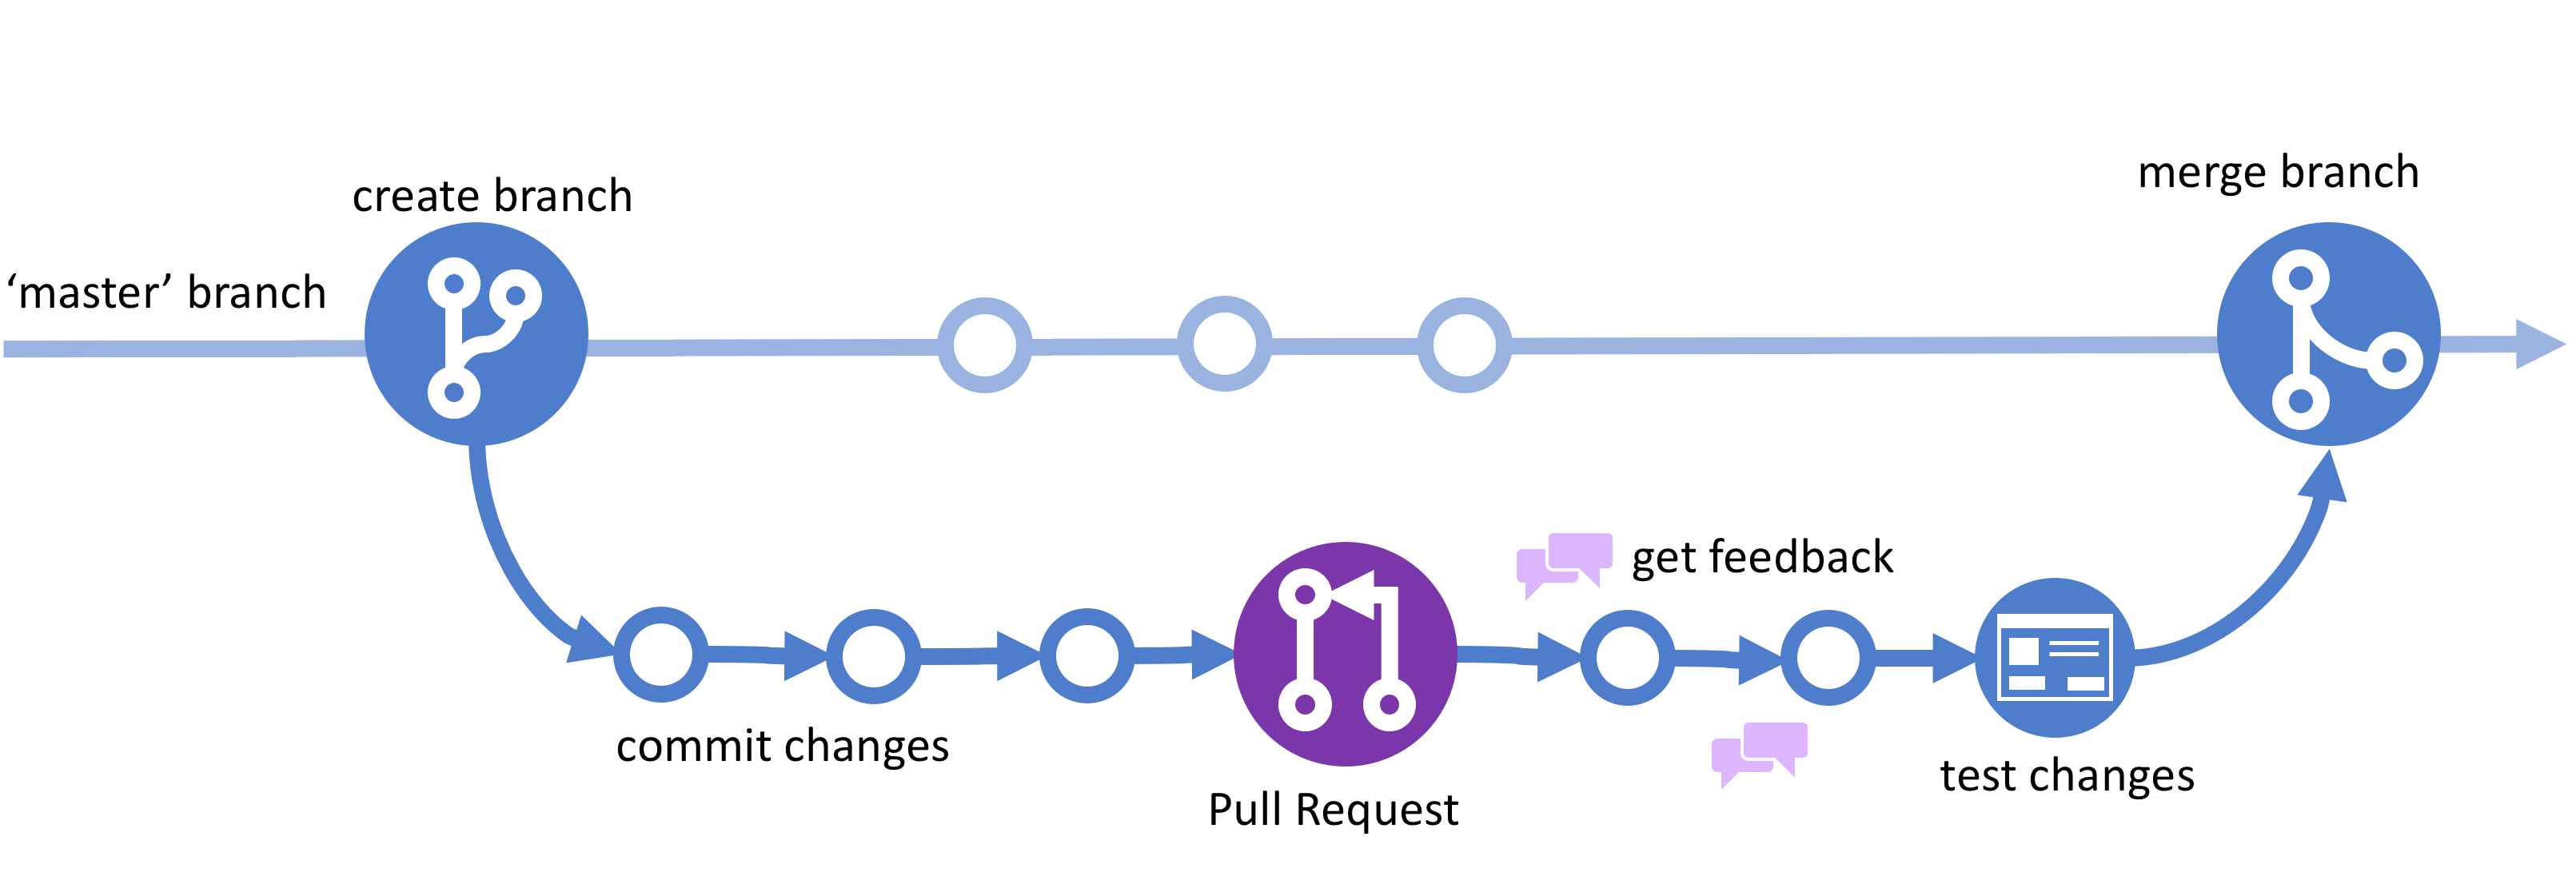
\includegraphics[width=1\textwidth]{../img/GitHub_Flow}
    ~\caption{GitHub Flow diagram.}
\end{figure}
\begin{itemize}
    \item \textbf{Master} -- is the branch we release code from and then deploy it to various environments like
    DEV, QA or UAT. Each state of master branch is deployable.
    \item \textbf{Feature} -- feature branch that created to implement new feature according to sprint plan.
    Feature branch is branched from the master's HEAD\@.
    \item \textbf{Bugfix} -- same as feature branch in general, branched out of master's HEAD and contains not critical bug fix.
    \item \textbf{Release/v*} -- branched from master and ready to be released, CD pipeline itself is triggered
    by push tag event from this branch.
    It is long-living branch used to support particular release.
    \item \textbf{Hotfix} -- branch is created from the latest deployed unit where error occurs,
    for example \texttt{release/v*} branch.
    Hotfixes are not stick to releases, they may be necessary in any deployed unit like DEV, QA environments,
    depends on where error occurs.
    This branch contains hotfix that should be deployed as soon as possible.
    In case of hotfix branch, release to be done directly from it.
    It means that after hotfix is finished new tag with patch increment to be created and pushed,
    triggering CI/CD and deployment of hotfix to production.
\end{itemize}

\subsection{Release process}
Having all above, assume we have current initial semantic version on our main branch as \texttt{v0.1.0},
and we must release upcoming version, our steps to perform are:
\begin{enumerate}
    \item Create pull request from recent \texttt{feature} branch to \texttt{master} branch, this pull request triggers
    Continuous Integration (CI) to start, CI runs tests, code quality checks etc.,
    but deployment won't be started yet, only CI\@.
    \item After all checks passed, pull request reviewed by team and every comment from code review is fixed -- pull
    request to be merged from \texttt{feature} branch to \texttt{master} branch.
    No CI/CD pipeline triggered by the merge.
    \item Next, responsible person reviews changes
    (using change log or git compare, it doesn't matter, but change log is preferable solution),
    responsible person makes decision which part of semantic version to increment and then creates
    and pushes tag to remote repository respectively.
    For example, it is decided that minor version should be incremented then our version becomes
    \texttt{v0.1.0 -> v0.2.0}, so responsible person creates release as follows:
    \begin{itemize}
        \item Checkout to branch \texttt{release/v0.2.0} from Master
        \item \texttt{git push origin release/v0.2.0}
        \item \texttt{git tag -a v0.2.0 -m "Release v0.2.0"}
        \item \texttt{git push origin v0.2.0}
    \end{itemize}
    \item After that CI/CD pipeline is triggered by tag push event~\cite{AzurePipelinesTriggers},
    after build there are three deployments scheduled: DEV, QA, UAT\@.
    Environments QA and UAT are to be approved by designated personnel before deployment starts,
    DEV to be deployed without manual approve.
    \item Finally, \texttt{master} branch cherry-picks from \texttt{release/v0.2.0} after deployment is complete.
\end{enumerate}
Entire process is shown on picture below
\begin{figure}[H]
    \centering
    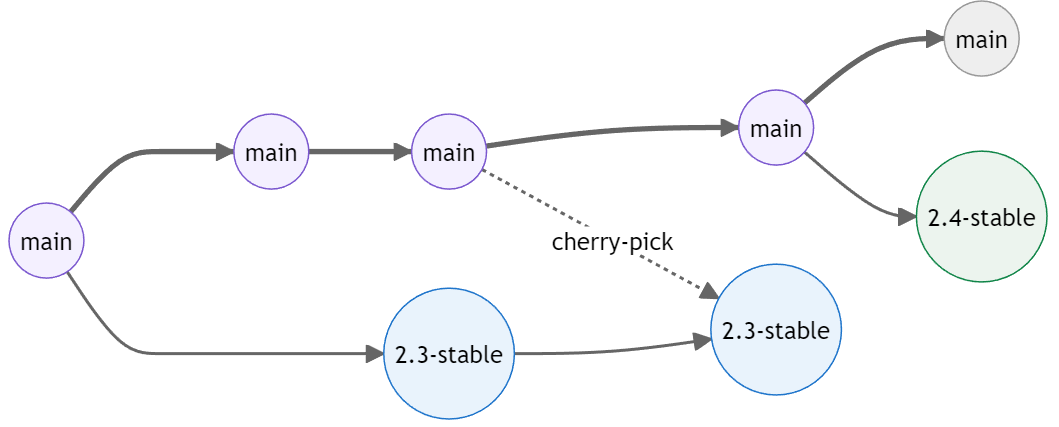
\includegraphics[width=1\textwidth]{../img/GitLab_Flow}
    ~\caption{GitLab Flow diagram~\cite{GitLabFlow}.}
\end{figure}


    \section{Conclusions}\label{sec:conclusions}
    Conclusions of your manuscript.

    \bibliographystyle{unsrt}
    \bibliography{ReleaseFlowProposal}
    \noindent \textbf{Version:} \texttt{Local-0.1.0}


\end{document}
